%\documentclass[ngerman,oneside]{cgsthesis}
\documentclass[ngerman]{cgsthesis}

\usepackage[utf8]{inputenc}

% Configure Biblatex

\usepackage[defernumbers=true,natbib=true,backend=bibtex,style=numeric]{biblatex}

% bug workaround, see http://tex.stackexchange.com/questions/311426/bibliography-error-use-of-blxbblverbaddi-doesnt-match-its-definition-ve
\makeatletter
\def\blx@maxline{77}
\makeatother
\DeclareBibliographyCategory{cited}
\DeclareBibliographyCategory{supplementary}
\AtEveryCitekey{\addtocategory{cited}{\thefield{entrykey}}}
\newcommand{\citesupplementary}[1]{\nocite{#1}\addtocategory{supplementary}{#1}}
\DefineBibliographyStrings{ngerman}{
  andothers = {\emph{et~al.}}
}
\DefineBibliographyStrings{english}{
  andothers = {\emph{et~al.}}
}
\addbibresource{foo-thesis.bib}

% Code listings

\usepackage{listings}
\lstloadlanguages{C++}
\usepackage{glsl}

% Thesis development

\usepackage{cgsnotes}
\usepackage{cgsparagraphclassification}

% Title page

\logo{graphics/logo_black}

\title{Titel der Arbeit}
%\subtitle{Untertitel} % z.B. englischer Titel bei Bachelorarbeit

%\subject{%
%    Bachelorarbeit\\
%    zur Erlangung des akademischen Grades\\
%    "Bachelor of Science"\\
%    (B.Sc.)\\
%    im Studiengang IT-Systems Engineering\\
%    des	 Hasso-Plattner-Instituts an der\\
%    Universit\"at Potsdam
%    \vfill
%    vorgelegt von}

%\subject{%
%    Masterarbeit\\
%    zur Erlangung des akademischen Grades\\
%    "Master of Science"\\
%    (M.Sc.)\\
%    im Studiengang IT-Systems Engineering\\
%    des	 Hasso-Plattner-Instituts an der\\
%    Universit\"at Potsdam
%    \vfill
%    vorgelegt von}

\subject{%
    Dissertation\\
    zur Erlangung des akademischen Grades\\
    "doctor rerum naturalium"\\
    (Dr.\ rer.\ nat.)\\
    in der Wissenschaftsdisziplin Informatik
    \vfill
    eingereicht an der\\
    Mathematisch-Naturwissenschaftlichen Fakult\"at\\
    der Universit\"at Potsdam\\
    \vfill
    von}

\author{Foo Bar}

%\publishers{%
%    Aufgabenstellung und Anleitung:\\
%    Prof.\ Dr.\ J\"urgen D\"ollner\\
%    Max Mustermann}

\place{Potsdam}
\date{\today}


\begin{document}

\frontmatter

\maketitle

\tableofcontents

%!TEX root = foo-thesis.tex

\chapter*{Abstract}
\addcontentsline{toc}{chapter}{Abstract}

\chapter*{Zusammenfassung}
\addcontentsline{toc}{chapter}{Zusammenfassung}

\cleardoublepage


\mainmatter
%!TEX root = foo-thesis.tex

\chapter{Einleitung}

Lorem ipsum dolor sit amet, consetetur sadipscing elitr, sed diam nonumy eirmod tempor invidunt ut labore et dolore magna aliquyam erat, sed diam voluptua. At vero eos et accusam et justo duo dolores et ea rebum. Stet clita kasd gubergren, no sea takimata sanctus est Lorem ipsum dolor sit amet. Lorem ipsum dolor sit amet, consetetur sadipscing elitr, sed diam nonumy eirmod tempor invidunt ut labore et dolore magna aliquyam erat, sed diam voluptua. At vero eos et accusam 
\begin{equation}
	\label{eq:testeqn}
	A = \sqrt{x^2 + y^2}
\end{equation}
et justo duo \cref{eq:testeqn} dolores et ea rebum. Stet clita kasd gubergren, no sea takimata sanctus est Lorem ipsum dolor sit amet. Lorem ipsum dolor sit amet, consetetur sadipscing elitr, sed diam nonumy eirmod tempor invidunt ut labore et dolore magna aliquyam erat, sed diam voluptua. \Cref{eq:testeqn} vero eos et accusam et justo duo dolores et ea rebum. Stet clita kasd gubergren, no sea takimata sanctus est Lorem ipsum dolor sit amet.   

Duis autem vel eum iriure dolor in hendrerit in vulputate velit esse molestie consequat, vel illum dolore eu feugiat nulla facilisis at vero eros et accumsan et iusto odio dignissim qui blandit praesent luptatum zzril delenit augue duis dolore te feugait nulla facilisi. Lorem ipsum dolor sit amet, consectetuer adipiscing elit, sed diam nonummy nibh euismod tincidunt ut laoreet dolore magna aliquam erat volutpat.   

Ut wisi enim ad minim veniam, quis nostrud exerci tation ullamcorper suscipit lobortis nisl ut aliquip ex ea commodo consequat. Duis autem vel eum iriure dolor in hendrerit in vulputate velit esse molestie consequat, vel illum dolore eu feugiat nulla facilisis at vero eros et accumsan et iusto odio dignissim qui blandit praesent luptatum zzril delenit augue duis dolore te feugait nulla facilisi.   


\section{General Related Work}

Lorem ipsum dolor sit amet, consetetur sadipscing elitr, sed diam nonumy eirmod tempor invidunt ut labore et dolore magna aliquyam erat, sed diam voluptua. At vero eos et accusam et justo duo dolores et ea rebum. Stet clita kasd gubergren, no sea takimata sanctus est Lorem ipsum dolor sit amet. Lorem ipsum dolor sit amet, consetetur sadipscing elitr, sed diam nonumy eirmod tempor invidunt ut labore et dolore magna aliquyam erat, sed diam voluptua. At vero eos et accusam et justo duo dolores et ea rebum. Stet clita kasd gubergren, no sea takimata sanctus est Lorem ipsum dolor sit amet. Lorem ipsum dolor sit amet, consetetur sadipscing elitr, sed diam nonumy eirmod tempor invidunt ut labore et dolore magna aliquyam erat, sed diam voluptua. At vero eos et accusam et justo duo dolores et ea rebum. Stet clita kasd gubergren, no sea takimata sanctus est Lorem ipsum dolor sit amet.   

Duis autem vel eum iriure dolor in hendrerit in vulputate velit esse molestie consequat, vel illum dolore eu feugiat nulla facilisis at vero eros et accumsan et iusto odio dignissim qui blandit praesent luptatum zzril delenit augue duis dolore te feugait nulla facilisi. Lorem ipsum dolor sit amet, consectetuer adipiscing elit, sed diam nonummy nibh euismod tincidunt ut laoreet dolore magna aliquam erat volutpat.   

Ut wisi enim ad minim veniam, quis nostrud exerci tation ullamcorper suscipit lobortis nisl ut aliquip ex ea commodo consequat. Duis autem vel eum iriure dolor in hendrerit in vulputate velit esse molestie consequat, vel illum dolore eu feugiat nulla facilisis at vero eros et accumsan et iusto odio dignissim qui blandit praesent luptatum zzril delenit augue duis dolore te feugait nulla facilisi.   

Nam liber tempor cum soluta nobis eleifend option congue nihil imperdiet doming id quod mazim placerat facer possim assum. Lorem ipsum dolor sit amet, consectetuer adipiscing elit, sed diam nonummy nibh euismod tincidunt ut laoreet dolore magna aliquam erat volutpat. Ut wisi enim ad minim veniam, quis nostrud exerci tation ullamcorper suscipit lobortis nisl ut aliquip ex ea commodo consequat.   

Duis autem vel eum iriure dolor in hendrerit in vulputate velit esse molestie consequat, vel illum dolore eu feugiat nulla facilisis.   

At vero eos et accusam et justo duo dolores et ea rebum. Stet clita kasd gubergren, no sea takimata sanctus est Lorem ipsum dolor sit amet. Lorem ipsum dolor sit amet, consetetur.


\section{Contributions}

Lorem ipsum dolor sit amet, consetetur sadipscing elitr, sed diam nonumy eirmod tempor invidunt ut labore et dolore magna aliquyam erat, sed diam voluptua. At vero eos et accusam et justo duo dolores et ea rebum. Stet clita kasd gubergren, no sea takimata sanctus est Lorem ipsum dolor sit amet. Lorem ipsum dolor sit amet, consetetur sadipscing elitr, sed diam nonumy eirmod tempor invidunt ut labore et dolore magna aliquyam erat, sed diam voluptua. At vero eos et accusam et justo duo dolores et ea rebum. Stet clita kasd gubergren, no sea takimata sanctus est Lorem ipsum dolor sit amet. Lorem ipsum dolor sit amet, consetetur sadipscing elitr, sed diam nonumy eirmod tempor invidunt ut labore et dolore magna aliquyam erat, sed diam voluptua. At vero eos et accusam et justo duo dolores et ea rebum. Stet clita kasd gubergren, no sea takimata sanctus est Lorem ipsum dolor sit amet.   

Duis autem vel eum iriure dolor in hendrerit in vulputate velit esse molestie consequat, vel illum dolore eu feugiat nulla facilisis at vero eros et accumsan et iusto odio dignissim qui blandit praesent luptatum zzril delenit augue duis dolore te feugait nulla facilisi. Lorem ipsum dolor sit amet, consectetuer adipiscing elit, sed diam nonummy nibh euismod tincidunt ut laoreet dolore magna aliquam erat volutpat.   

Ut wisi enim ad minim veniam, quis nostrud exerci tation ullamcorper suscipit lobortis nisl ut aliquip ex ea commodo consequat. Duis autem vel eum iriure dolor in hendrerit in vulputate velit esse molestie consequat, vel illum dolore eu feugiat nulla facilisis at vero eros et accumsan et iusto odio dignissim qui blandit praesent luptatum zzril delenit augue duis dolore te feugait nulla facilisi.   

Nam liber tempor cum soluta nobis eleifend option congue nihil imperdiet doming id quod mazim placerat facer possim assum. Lorem ipsum dolor sit amet, consectetuer adipiscing elit, sed diam nonummy nibh euismod tincidunt ut laoreet dolore magna aliquam erat volutpat. Ut wisi enim ad minim veniam, quis nostrud exerci tation ullamcorper suscipit lobortis nisl ut aliquip ex ea commodo consequat.   

Duis autem vel eum iriure dolor in hendrerit in vulputate velit esse molestie consequat, vel illum dolore eu feugiat nulla facilisis.   

At vero eos et accusam et justo duo dolores et ea rebum. Stet clita kasd gubergren, no sea takimata sanctus est Lorem ipsum dolor sit amet. Lorem ipsum dolor sit amet, consetetur


\section{Application Areas}

Lorem ipsum dolor sit amet, consetetur sadipscing elitr, sed diam nonumy eirmod tempor invidunt ut labore et dolore magna aliquyam erat, sed diam voluptua. At vero eos et accusam et justo duo dolores et ea rebum. Stet clita kasd gubergren, no sea takimata sanctus est Lorem ipsum dolor sit amet. Lorem ipsum dolor sit amet, consetetur sadipscing elitr, sed diam nonumy eirmod tempor invidunt ut labore et dolore magna aliquyam erat, sed diam voluptua. At vero eos et accusam et justo duo dolores et ea rebum. Stet clita kasd gubergren, no sea takimata sanctus est Lorem ipsum dolor sit amet. Lorem ipsum dolor sit amet, consetetur sadipscing elitr, sed diam nonumy eirmod tempor invidunt ut labore et dolore magna aliquyam erat, sed diam voluptua. At vero eos et accusam et justo duo dolores et ea rebum. Stet clita kasd gubergren, no sea takimata sanctus est Lorem ipsum dolor sit amet.   

Duis autem vel eum iriure dolor in hendrerit in vulputate velit esse molestie consequat, vel illum dolore eu feugiat nulla facilisis at vero eros et accumsan et iusto odio dignissim qui blandit praesent luptatum zzril delenit augue duis dolore te feugait nulla facilisi. Lorem ipsum dolor sit amet, consectetuer adipiscing elit, sed diam nonummy nibh euismod tincidunt ut laoreet dolore magna aliquam erat volutpat.   

Ut wisi enim ad minim veniam, quis nostrud exerci tation ullamcorper suscipit lobortis nisl ut aliquip ex ea commodo consequat. Duis autem vel eum iriure dolor in hendrerit in vulputate velit esse molestie consequat, vel illum dolore eu feugiat nulla facilisis at vero eros et accumsan et iusto odio dignissim qui blandit praesent luptatum zzril delenit augue duis dolore te feugait nulla facilisi.   

Nam liber tempor cum soluta nobis eleifend option congue nihil imperdiet doming id quod mazim placerat facer possim assum. Lorem ipsum dolor sit amet, consectetuer adipiscing elit, sed diam nonummy nibh euismod tincidunt ut laoreet dolore magna aliquam erat volutpat. Ut wisi enim ad minim veniam, quis nostrud exerci tation ullamcorper suscipit lobortis nisl ut aliquip ex ea commodo consequat.   

\cleardoublepage

% !TeX root = foo-thesis.tex

\chapter{Erstes Hauptteil Kapitel}

Lorem ipsum dolor sit amet, consetetur sadipscing elitr, sed diam nonumy eirmod tempor invidunt ut labore et dolore magna aliquyam erat, sed diam voluptua. At vero eos et accusam et justo duo dolores et ea rebum. Stet clita kasd gubergren, no sea takimata sanctus est Lorem ipsum dolor sit amet. Lorem ipsum dolor sit amet, consetetur sadipscing elitr, sed diam nonumy eirmod tempor invidunt ut labore et dolore magna aliquyam erat, sed diam voluptua. At vero eos et accusam et justo duo dolores et ea rebum. Stet clita kasd gubergren, no sea takimata sanctus est Lorem ipsum dolor sit amet. Lorem ipsum dolor sit amet, consetetur sadipscing elitr, sed diam nonumy eirmod tempor invidunt ut labore et \citep{Aubert.Kornprobst-2006} dolore magna aliquyam erat, sed diam voluptua. At vero eos et accusam et justo duo dolores et ea rebum. Stet clita kasd gubergren, no sea takimata sanctus est Lorem ipsum dolor sit amet.

Duis autem vel eum iriure dolor in hendrerit in vulputate velit esse molestie consequat, vel illum dolore eu feugiat nulla facilisis at vero eros et accumsan et iusto odio dignissim qui blandit praesent luptatum zzril delenit augue duis dolore te feugait nulla facilisi. Lorem ipsum dolor sit amet, consectetuer adipiscing elit, sed diam nonummy nibh euismod tincidunt ut laoreet dolore magna aliquam erat volutpat.
Ut wisi enim ad minim veniam, quis nostrud exerci tation ullamcorper suscipit lobortis nisl ut aliquip ex ea commodo consequat. Duis autem vel eum iriure dolor in hendrerit in vulputate velit esse molestie consequat, vel illum dolore eu feugiat nulla facilisis at vero eros et accumsan et iusto odio dignissim qui blandit praesent luptatum zzril delenit augue duis dolore te feugait nulla facilisi.
Nam liber tempor cum soluta nobis eleifend option congue nihil imperdiet doming id quod mazim placerat facer possim assum. Lorem ipsum dolor sit amet, consectetuer adipiscing elit, sed diam nonummy nibh euismod tincidunt ut laoreet dolore magna aliquam erat volutpat. Ut wisi enim ad minim veniam, quis nostrud exerci tation ullamcorper suscipit lobortis nisl ut aliquip ex ea commodo consequat.


\section{Aat accusam aliquyam diam}
Duis autem vel eum iriure dolor in hendrerit in vulputate velit esse molestie consequat, vel illum dolore eu feugiat nulla facilisis.
At vero eos et accusam et justo duo dolores et ea rebum. Stet clita kasd gubergren, no sea takimata sanctus est Lorem ipsum dolor sit amet. Lorem ipsum dolor sit amet, consetetur sadipscing elitr, sed diam nonumy eirmod tempor invidunt ut labore et dolore magna aliquyam erat, sed diam voluptua. At vero eos et accusam et justo duo dolores et ea rebum. Stet clita kasd gubergren, no sea takimata sanctus est Lorem ipsum dolor sit amet. Lorem ipsum dolor sit amet, consetetur sadipscing elitr, At accusam aliquyam diam diam dolore dolores duo eirmod eos erat, et nonumy sed tempor et et invidunt justo labore Stet clita ea et gubergren, kasd magna no rebum. sanctus sea sed takimata ut vero voluptua. est Lorem ipsum dolor sit amet. Lorem ipsum dolor sit amet, consetetur sadipscing elitr, sed diam nonumy eirmod tempor invidunt ut labore et dolore magna aliquyam erat.


\subsection{Stet clita kasd gubergren}
Consetetur \citep{Goshtasby.Satter-2008} sadipscing elitr, sed diam nonumy eirmod tempor invidunt ut labore et dolore magna aliquyam erat, sed diam voluptua. At vero eos et accusam et justo duo dolores et ea rebum. Stet clita kasd gubergren, no sea takimata sanctus est Lorem ipsum dolor sit amet. Lorem ipsum dolor sit amet, consetetur sadipscing elitr, sed diam nonumy eirmod tempor invidunt ut labore et dolore magna aliquyam erat, sed diam voluptua. At vero eos et accusam et justo duo dolores et ea rebum. Stet clita kasd gubergren, no sea takimata sanctus est Lorem ipsum dolor sit amet. Lorem ipsum dolor sit amet, consetetur sadipscing elitr, sed diam nonumy eirmod tempor invidunt ut labore et dolore magna aliquyam erat, sed diam voluptua. At vero eos et accusam et justo duo dolores et ea rebum. Stet clita kasd gubergren, no sea takimata sanctus.
\begin{itemize}
\item Duis autem vel eum iriure dolor in hendrerit in vulputate velit esse molestie consequat, vel illum dolore eu feugiat nulla facilisis at vero eros et
\item Et iusto odio dignissim qui blandit praesent luptatum zzril delenit augue duis dolore te feugait nulla facilisi. Lorem ipsum dolor sit.
\begin{itemize}
\item Duis autem vel eum iriure dolor in hendrerit in vulputate velit esse molestie consequat, vel illum dolore eu feugiat nulla facilisis at vero eros et.
\item Et iusto odio dignissim qui blandit praesent luptatum zzril delenit augue duis dolore te feugait nulla facilisi. Lorem ipsum dolor sit.
\item Amet, consectetuer adipiscing elit, sed diam nonummy nibh euismod tincidunt ut laoreet dolore magna aliquam erat volutpat.
\end{itemize}
\item Amet, consectetuer adipiscing elit, sed diam nonummy nibh euismod tincidunt ut laoreet dolore magna aliquam erat volutpat.
\end{itemize}
Lorem ipsum dolor sit amet, consetetur sadipscing elitr, sed diam nonumy eirmod tempor invidunt ut labore et dolore magna aliquyam erat, sed diam voluptua. At vero eos et accusam et justo duo dolores et ea rebum. Stet clita kasd gubergren, no sea takimata sanctus est Lorem ipsum dolor sit amet. Lorem ipsum dolor sit amet, consetetur sadipscing elitr, sed diam nonumy eirmod tempor invidunt ut labore et dolore magna aliquyam erat, sed diam voluptua. At vero eos et accusam et justo duo dolores et ea rebum. Stet clita kasd gubergren, no sea takimata sanctus est Lorem ipsum dolor sit amet. Lorem ipsum dolor sit amet, consetetur sadipscing elitr, sed diam nonumy eirmod tempor invidunt ut labore et dolore magna aliquyam erat, sed diam voluptua. At vero eos et accusam et justo duo dolores et ea rebum. Stet clita kasd gubergren, no sea takimata sanctus est Lorem ipsum dolor sit amet.
Duis autem vel eum iriure dolor in hendrerit in vulputate velit esse molestie consequat, vel illum dolore eu feugiat nulla facilisis at vero eros et accumsan et iusto odio dignissim qui blandit praesent luptatum zzril delenit augue duis dolore te feugait nulla facilisi. Lorem ipsum dolor sit amet, consectetuer adipiscing elit, sed diam nonummy nibh euismod tincidunt ut laoreet dolore magna aliquam erat volutpat.
Ut wisi enim ad minim veniam, quis nostrud exerci tation ullamcorper suscipit lobortis nisl ut aliquip ex ea commodo consequat. Duis autem vel eum iriure dolor in hendrerit in vulputate velit esse molestie consequat, vel illum dolore eu feugiat nulla facilisis at vero eros et accumsan et iusto odio dignissim qui blandit praesent luptatum zzril delenit augue duis dolore te feugait nulla facilisi.

\subsection{Stet clita kasd gubergren}
Nam liber tempor cum soluta nobis eleifend option congue nihil imperdiet doming id quod mazim placerat facer possim assum. Lorem ipsum dolor sit amet, consectetuer adipiscing elit, sed diam nonummy nibh euismod tincidunt ut laoreet dolore magna aliquam erat volutpat. Ut wisi enim ad minim veniam, quis nostrud exerci tation ullamcorper suscipit lobortis nisl ut aliquip ex ea commodo consequat.
Duis autem vel eum iriure dolor in hendrerit in vulputate velit esse molestie consequat, vel illum dolore eu feugiat nulla facilisis.
At vero eos et accusam et justo duo dolores et ea rebum. Stet clita kasd gubergren, no sea takimata sanctus est Lorem ipsum dolor sit amet. Lorem ipsum dolor sit amet, consetetur sadipscing elitr, sed diam nonumy eirmod tempor invidunt ut labore et dolore magna aliquyam erat, sed diam voluptua. At vero eos et accusam et justo duo dolores et ea rebum. Stet clita kasd gubergren, no sea takimata sanctus est Lorem ipsum dolor sit amet. Lorem ipsum dolor sit amet, consetetur sadipscing elitr, At accusam aliquyam diam diam dolore dolores duo eirmod eos erat, et nonumy sed tempor et et invidunt justo labore Stet clita ea et gubergren, kasd magna no rebum. sanctus sea sed takimata ut vero voluptua. est Lorem ipsum dolor sit amet. Lorem ipsum dolor sit amet, consetetur sadipscing elitr, sed diam nonumy eirmod tempor invidunt ut labore et dolore magna aliquyam erat.

\begin{figure}
    \includegraphics[width=\textwidth]{graphics/test3}
    \caption{Stet clita kasd gubergren, no sea takimata sanctus est Lorem ipsum dolor sit amet. Lorem ipsum dolor sit amet, consetetur sadipscing elitr.}
\end{figure}

Consetetur sadipscing elitr, \citep{Yang.etal-1996} sed diam nonumy eirmod tempor invidunt ut labore et dolore magna aliquyam erat, sed diam voluptua. At vero eos et accusam et justo duo dolores et ea rebum. Stet clita kasd gubergren, no sea takimata sanctus est Lorem ipsum dolor sit amet. Lorem ipsum dolor sit amet, consetetur sadipscing elitr, sed diam nonumy eirmod tempor invidunt ut labore et dolore magna aliquyam erat, sed diam voluptua. At vero eos et accusam et justo duo dolores et ea rebum. Stet clita kasd gubergren, no sea takimata sanctus est Lorem ipsum dolor sit amet. Lorem ipsum dolor sit amet, consetetur sadipscing elitr, sed diam nonumy eirmod tempor invidunt ut labore et dolore magna aliquyam erat, sed diam voluptua. At vero eos et accusam et justo duo dolores et ea rebum. Stet clita kasd gubergren, no sea takimata sanctus.


\subsection{At vero eos et accusam}
Lorem ipsum dolor sit amet, consetetur sadipscing elitr, sed diam nonumy eirmod tempor invidunt ut labore et dolore magna aliquyam erat, sed diam voluptua. At vero eos et accusam et justo duo dolores et ea rebum. Stet clita kasd gubergren, no sea takimata sanctus est Lorem ipsum dolor sit amet. Lorem ipsum dolor sit amet, consetetur sadipscing elitr, sed diam nonumy eirmod tempor invidunt ut labore et dolore magna aliquyam erat, sed diam voluptua. At vero eos et accusam et justo duo dolores et ea rebum. Stet clita kasd gubergren, no sea takimata sanctus est Lorem ipsum dolor sit amet. Lorem ipsum dolor sit amet, consetetur sadipscing elitr, sed diam nonumy eirmod tempor invidunt ut labore et dolore magna aliquyam erat, sed diam voluptua. At vero eos et accusam et justo duo dolores et ea rebum. Stet clita kasd gubergren, no sea takimata sanctus est Lorem ipsum dolor sit amet.
Duis autem vel eum iriure dolor in hendrerit in vulputate velit esse molestie consequat, vel illum dolore eu feugiat nulla facilisis at vero eros et accumsan et iusto odio dignissim qui blandit praesent luptatum zzril delenit augue duis dolore te feugait nulla facilisi. Lorem ipsum dolor sit amet, consectetuer adipiscing elit, sed diam nonummy nibh euismod tincidunt ut laoreet dolore magna aliquam erat volutpat.

Ut wisi enim ad minim veniam, quis nostrud exerci tation ullamcorper suscipit lobortis nisl ut aliquip ex ea commodo consequat. Duis autem vel eum iriure dolor in hendrerit in vulputate velit esse molestie consequat, vel illum dolore eu feugiat \citep{Guichard.Morel-2003} nulla facilisis at vero eros et accumsan et iusto odio dignissim qui blandit praesent luptatum zzril delenit augue duis dolore te feugait nulla facilisi.
Nam liber tempor cum soluta nobis eleifend option congue nihil imperdiet doming id quod mazim placerat facer possim assum. Lorem ipsum dolor sit amet, consectetuer adipiscing elit, sed diam nonummy nibh euismod tincidunt ut laoreet dolore magna aliquam erat volutpat. Ut wisi enim ad minim veniam, quis nostrud exerci tation ullamcorper suscipit lobortis nisl ut aliquip ex ea commodo consequat.
Duis autem vel eum iriure dolor in hendrerit in vulputate velit esse molestie consequat, vel illum dolore eu feugiat nulla facilisis.

\begin{figure}
    \centering%
    \includegraphics[width=0.32\textwidth]{graphics/test0}
    \caption{Stet clita kasd gubergren, no sea takimata sanctus est.}
\end{figure}


\section{At accusam aliquyam}
At vero eos et accusam et justo duo dolores et ea rebum. Stet clita kasd gubergren, no sea takimata sanctus est Lorem ipsum dolor sit amet. Lorem ipsum dolor sit amet, consetetur sadipscing elitr, sed diam nonumy eirmod tempor invidunt ut labore et dolore magna aliquyam erat, sed diam voluptua. At vero eos et accusam et justo duo dolores et ea rebum. Stet clita kasd gubergren, no sea takimata sanctus est Lorem ipsum dolor sit amet. Lorem ipsum dolor sit amet, consetetur sadipscing elitr, At accusam aliquyam diam diam dolore dolores duo eirmod eos erat, et nonumy sed tempor et et invidunt justo labore Stet clita ea et gubergren, kasd magna no rebum. sanctus sea sed takimata ut vero voluptua. est Lorem ipsum dolor sit amet. Lorem ipsum dolor sit amet, consetetur sadipscing elitr, sed diam nonumy eirmod tempor invidunt ut labore et dolore magna aliquyam erat.
\begin{itemize}
\item Duis autem vel eum iriure dolor in hendrerit in vulputate velit esse molestie consequat, vel illum dolore eu feugiat nulla facilisis at vero eros et
\item Et iusto odio dignissim qui blandit praesent luptatum zzril delenit augue duis dolore te feugait nulla facilisi. Lorem ipsum dolor sit.
\item Amet, consectetuer adipiscing elit, sed diam nonummy nibh euismod tincidunt ut laoreet dolore magna aliquam erat volutpat.
\end{itemize}

Consetetur sadipscing elitr, \citep{Barash.Comaniciu-2004} sed diam nonumy eirmod tempor invidunt ut labore et dolore magna aliquyam erat, sed diam voluptua. At vero eos et accusam et justo duo dolores et ea rebum. Stet clita kasd gubergren, no sea takimata sanctus est Lorem ipsum dolor sit amet. Lorem ipsum dolor sit amet, consetetur sadipscing elitr, sed diam nonumy eirmod tempor invidunt ut labore et dolore magna aliquyam erat, sed diam voluptua. At vero eos et accusam et justo duo dolores et ea rebum. Stet clita kasd gubergren, no sea takimata sanctus est Lorem ipsum dolor sit amet. Lorem ipsum dolor sit amet, consetetur sadipscing elitr, sed diam nonumy eirmod tempor invidunt ut labore et dolore magna aliquyam erat, sed diam voluptua. At vero eos et accusam et justo duo dolores et ea rebum. Stet clita kasd gubergren, no sea takimata sanctus.
Lorem ipsum dolor sit amet, consetetur sadipscing elitr, sed diam nonumy eirmod tempor invidunt ut labore et dolore magna aliquyam erat, sed diam voluptua. At vero eos et accusam et justo duo dolores et ea rebum. Stet clita kasd gubergren, no sea takimata sanctus est Lorem ipsum dolor sit amet. Lorem ipsum dolor sit amet, consetetur sadipscing elitr, sed diam nonumy eirmod tempor invidunt ut labore et dolore magna aliquyam erat, sed diam voluptua. At vero eos et accusam et justo duo dolores et ea rebum. Stet clita kasd gubergren, no sea takimata sanctus est Lorem ipsum dolor sit amet. Lorem ipsum dolor sit amet, consetetur sadipscing elitr, sed diam nonumy eirmod tempor invidunt ut labore et dolore magna aliquyam erat, sed diam voluptua. At vero eos et accusam et justo duo dolores et ea rebum. Stet clita kasd gubergren, no sea takimata sanctus est Lorem ipsum dolor sit amet.
Duis autem vel eum iriure dolor in hendrerit in vulputate velit esse molestie consequat, vel illum dolore eu feugiat nulla facilisis at vero eros et accumsan et iusto odio dignissim qui blandit praesent luptatum zzril delenit augue duis dolore te feugait nulla facilisi. Lorem ipsum dolor sit amet, consectetuer adipiscing elit, sed diam nonummy nibh euismod tincidunt ut laoreet dolore magna aliquam erat volutpat.

\begin{figure}
    \subcaptionbox{\label{fig:test3a}Test 1}{\includegraphics[width=0.32\textwidth]{graphics/test0}}%
    \hfill%
    \subcaptionbox{\label{fig:test3b}Test 2}{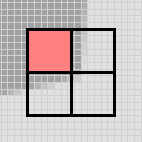
\includegraphics[width=0.32\textwidth]{graphics/test1}}%
    \hfill%
    \subcaptionbox{\label{fig:test3c}Test 3}{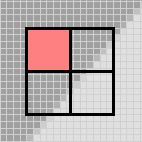
\includegraphics[width=0.32\textwidth]{graphics/test2}}%
    \caption{Stet clita kasd gubergren, no sea takimata}
    \label{fig:test3}
\end{figure}

\textbf{Ut wisi enim} ad minim veniam, quis nostrud exerci tation ullamcorper suscipit lobortis nisl ut aliquip ex ea commodo consequat. Duis autem vel eum iriure dolor in hendrerit in vulputate velit esse molestie consequat, vel illum dolore eu feugiat nulla facilisis at vero eros et accumsan et iusto odio dignissim qui blandit praesent luptatum zzril delenit augue duis dolore te feugait nulla facilisi.
Nam liber tempor cum soluta nobis eleifend option congue nihil imperdiet doming id quod mazim placerat facer possim assum. Lorem ipsum dolor sit amet, consectetuer adipiscing elit, sed diam nonummy nibh euismod tincidunt ut laoreet dolore magna aliquam erat volutpat. Ut wisi enim ad minim veniam, quis nostrud exerci tation ullamcorper suscipit lobortis nisl ut aliquip ex ea commodo consequat.
Duis autem vel eum iriure dolor in hendrerit in vulputate velit esse molestie consequat, vel illum dolore eu feugiat nulla facilisis.

At vero eos et accusam et \citep{Black.Rangarajan-1996} justo duo dolores et ea rebum. Stet clita kasd gubergren, no sea takimata sanctus est Lorem ipsum dolor sit amet. Lorem ipsum dolor sit amet, consetetur sadipscing elitr, sed diam nonumy eirmod tempor invidunt ut labore et dolore magna aliquyam erat, sed diam voluptua. At vero eos et accusam et justo duo dolores et ea rebum. Stet clita kasd gubergren, no sea takimata sanctus est Lorem ipsum dolor sit amet. Lorem ipsum dolor sit amet, consetetur sadipscing elitr, At accusam aliquyam diam diam dolore dolores duo eirmod eos erat, et nonumy sed tempor et et invidunt justo labore Stet clita ea et gubergren, kasd magna no rebum. sanctus sea sed takimata ut vero voluptua. est Lorem ipsum dolor sit amet. Lorem ipsum dolor sit amet, consetetur sadipscing elitr, sed diam nonumy eirmod tempor invidunt ut labore et dolore magna aliquyam erat.

Referenzieren von Abbildungen: Abbildunng~\ref{fig:test3}, Abbildung~\ref{fig:test3a}, Abbildung~\ref{fig:test3}\subref{fig:test3a}-\subref{fig:test3c}.

Consetetur sadipscing elitr, sed diam nonumy eirmod tempor invidunt ut labore et dolore magna aliquyam erat, sed diam voluptua. At vero eos et accusam et justo duo dolores et ea rebum. Stet clita kasd gubergren, no sea takimata sanctus est Lorem ipsum dolor sit amet. Lorem ipsum dolor sit amet, consetetur sadipscing elitr, sed diam nonumy eirmod tempor invidunt ut labore et dolore magna aliquyam erat, sed diam voluptua. At vero eos et accusam et justo duo dolores et ea rebum. Stet clita kasd gubergren, no sea takimata sanctus est Lorem ipsum dolor sit amet. Lorem ipsum dolor sit amet, consetetur sadipscing elitr, sed diam nonumy eirmod tempor invidunt ut labore et dolore magna aliquyam erat, sed diam voluptua. At vero eos et accusam et justo duo dolores et ea rebum. Stet clita kasd gubergren, no sea takimata sanctus.

Lorem ipsum dolor sit amet, consetetur sadipscing elitr, sed diam nonumy eirmod tempor invidunt ut labore et dolore magna aliquyam erat, sed diam voluptua. At vero eos et accusam et justo duo dolores et ea rebum. Stet clita kasd gubergren, no sea takimata sanctus est Lorem ipsum dolor sit amet. Lorem ipsum dolor sit amet, consetetur sadipscing elitr, sed diam nonumy eirmod tempor invidunt ut labore et dolore magna aliquyam erat, sed diam voluptua. At vero eos et accusam et justo duo dolores et ea rebum. Stet clita kasd gubergren, no sea takimata sanctus est Lorem ipsum dolor sit amet. Lorem ipsum dolor sit amet, consetetur sadipscing elitr, sed diam nonumy eirmod tempor invidunt ut labore et dolore magna aliquyam erat, sed diam voluptua. At vero eos et accusam et justo duo dolores et ea rebum. Stet clita kasd gubergren, no sea takimata sanctus est Lorem ipsum dolor sit amet.
Duis autem vel eum iriure dolor in hendrerit in vulputate velit esse molestie consequat, vel illum dolore eu feugiat nulla facilisis at vero eros et accumsan et iusto odio dignissim qui blandit praesent luptatum zzril delenit augue duis dolore te feugait nulla facilisi. Lorem ipsum dolor sit amet, consectetuer adipiscing elit, sed diam nonummy nibh euismod tincidunt ut laoreet dolore magna aliquam erat volutpat.
Ut wisi enim ad minim veniam, quis nostrud exerci tation ullamcorper suscipit lobortis nisl ut aliquip ex ea commodo consequat. Duis autem vel eum iriure dolor in hendrerit in vulputate velit esse molestie consequat, vel illum dolore eu feugiat nulla facilisis at vero eros et accumsan et iusto odio dignissim qui blandit praesent luptatum zzril delenit augue duis dolore te feugait nulla facilisi.
Nam liber tempor cum soluta nobis eleifend option congue nihil imperdiet doming id quod mazim placerat facer possim assum. Lorem ipsum dolor sit amet, consectetuer adipiscing elit, sed diam nonummy nibh euismod tincidunt ut laoreet dolore magna aliquam erat volutpat. Ut wisi enim ad minim veniam, quis nostrud exerci tation ullamcorper suscipit lobortis nisl ut aliquip ex ea commodo consequat.
Duis autem vel eum iriure dolor in hendrerit in vulputate velit esse molestie consequat, vel illum dolore eu feugiat nulla facilisis.

\lstinputlisting[float,caption={Consetetur sadipscing elitr, sed diam nonumy eirmod tempor invidunt ut labore et dolore magna.}]{graphics/bf.glsl}%

At vero eos et accusam et justo duo dolores et ea rebum. Stet clita kasd gubergren, no sea takimata sanctus est Lorem ipsum dolor sit amet. Lorem ipsum dolor sit amet, consetetur sadipscing elitr, sed diam nonumy eirmod tempor invidunt ut labore et dolore magna aliquyam erat, sed diam voluptua. At vero eos et accusam et justo duo dolores et ea rebum. Stet clita kasd gubergren, no sea takimata sanctus est Lorem ipsum dolor sit amet. Lorem ipsum dolor sit amet, consetetur sadipscing elitr, At accusam aliquyam diam diam dolore dolores duo eirmod eos erat, et nonumy sed tempor et et invidunt justo labore Stet clita ea et gubergren, kasd magna no rebum. sanctus sea sed takimata ut vero voluptua. est Lorem ipsum dolor sit amet. Lorem ipsum dolor sit amet, consetetur sadipscing elitr, sed diam nonumy eirmod tempor invidunt ut labore et dolore magna aliquyam erat.

Consetetur sadipscing elitr, sed diam nonumy eirmod tempor invidunt ut labore et dolore magna aliquyam erat, sed diam voluptua. At vero eos et accusam et justo duo dolores et ea rebum. Stet clita kasd gubergren, no sea takimata sanctus est Lorem ipsum dolor sit amet. Lorem ipsum dolor sit amet, consetetur sadipscing elitr, sed diam nonumy eirmod tempor invidunt ut labore et dolore magna aliquyam erat, sed diam voluptua. At vero eos et accusam et justo duo dolores et ea rebum. Stet clita kasd gubergren, no sea takimata sanctus est Lorem ipsum dolor sit amet. Lorem ipsum dolor sit amet, consetetur sadipscing elitr, sed diam nonumy eirmod tempor invidunt ut labore et dolore magna aliquyam erat, sed diam voluptua. At vero eos et accusam et justo duo dolores et ea rebum. Stet clita kasd gubergren, no sea takimata sanctus.

Lorem ipsum dolor sit amet, consetetur sadipscing elitr, sed diam nonumy eirmod tempor invidunt ut labore et dolore magna aliquyam erat, sed diam voluptua. At vero eos et accusam et justo duo dolores et ea rebum. Stet clita kasd gubergren, no sea takimata sanctus est Lorem ipsum dolor sit amet. Lorem ipsum dolor sit amet, consetetur sadipscing elitr, sed diam nonumy eirmod tempor invidunt ut labore et dolore magna aliquyam erat, sed diam voluptua. At vero eos et accusam et justo duo dolores et ea rebum. Stet clita kasd gubergren, no sea takimata sanctus est Lorem ipsum dolor sit amet. Lorem ipsum dolor sit amet, consetetur sadipscing elitr, sed diam nonumy eirmod tempor invidunt ut labore et dolore magna aliquyam erat, sed diam voluptua. At vero eos et accusam et justo duo dolores et ea rebum. Stet clita kasd gubergren, no sea takimata sanctus est Lorem ipsum dolor sit amet.
Duis autem vel eum iriure dolor in hendrerit in vulputate velit esse molestie consequat, vel illum dolore eu feugiat nulla facilisis at vero eros et accumsan et iusto odio dignissim qui blandit praesent luptatum zzril delenit augue duis dolore te feugait nulla facilisi. Lorem ipsum dolor sit amet, consectetuer adipiscing elit, sed diam nonummy nibh euismod tincidunt ut laoreet dolore magna aliquam erat volutpat.

\begin{figure}
    \subcaptionbox{Test 1}{\includegraphics[width=0.32\textwidth]{graphics/test0}}%
    \hfill%
    \subcaptionbox{Test 2}{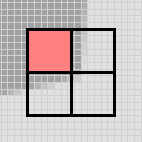
\includegraphics[width=0.32\textwidth]{graphics/test1}}%
    \hfill%
    \subcaptionbox{Test 3}{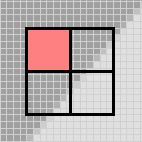
\includegraphics[width=0.32\textwidth]{graphics/test2}}%
    \par\medskip%
    \subcaptionbox{Test 1}{\includegraphics[width=0.32\textwidth]{graphics/test0}}%
    \hfill%
    \subcaptionbox{Test 2}{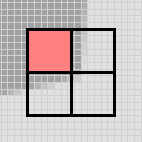
\includegraphics[width=0.32\textwidth]{graphics/test1}}%
    \hfill%
    \subcaptionbox{Test 3}{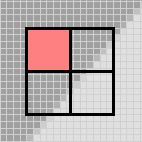
\includegraphics[width=0.32\textwidth]{graphics/test2}}%
    \caption{Stet clita kasd gubergren, no sea takimata sanctus est. Stet clita kasd gubergren, no sea takimata sanctus est.}
\end{figure}

Ut wisi enim ad minim veniam, quis nostrud exerci tation ullamcorper suscipit lobortis nisl ut aliquip ex ea commodo consequat. Duis autem vel eum iriure dolor in hendrerit in vulputate velit esse molestie consequat, vel illum dolore eu feugiat nulla facilisis at vero eros et accumsan et iusto odio dignissim qui blandit praesent luptatum zzril delenit augue duis dolore te feugait nulla facilisi.
Nam liber tempor cum soluta nobis eleifend option congue nihil imperdiet doming id quod mazim placerat facer possim assum. Lorem ipsum dolor sit amet, consectetuer adipiscing elit, sed diam nonummy nibh euismod tincidunt ut laoreet dolore magna aliquam erat volutpat. Ut wisi enim ad minim veniam, quis nostrud exerci tation ullamcorper suscipit lobortis nisl ut aliquip ex ea commodo consequat.
Duis autem vel eum iriure dolor in hendrerit in vulputate velit esse molestie consequat, vel illum dolore eu feugiat nulla facilisis.

At vero eos et accusam et justo duo dolores et ea rebum. Stet clita kasd gubergren, no sea takimata sanctus est Lorem ipsum dolor sit amet. Lorem ipsum dolor sit amet, consetetur sadipscing elitr, sed diam nonumy eirmod tempor invidunt ut labore et dolore magna aliquyam erat, sed diam voluptua. At vero eos et accusam et justo duo dolores et ea rebum. Stet clita kasd gubergren, no sea takimata sanctus est Lorem ipsum dolor sit amet. Lorem ipsum dolor sit amet, consetetur sadipscing elitr, At accusam aliquyam diam diam dolore dolores duo eirmod eos erat, et nonumy sed tempor et et invidunt justo labore Stet clita ea et gubergren, kasd magna no rebum. sanctus sea sed takimata ut vero voluptua. est Lorem ipsum dolor sit amet. Lorem ipsum dolor sit amet, consetetur sadipscing elitr, sed diam nonumy eirmod tempor invidunt ut labore et dolore magna aliquyam erat.
Consetetur sadipscing elitr, sed diam nonumy eirmod tempor invidunt ut labore et dolore magna aliquyam erat, sed diam voluptua. At vero eos et accusam et justo duo dolores et ea rebum. Stet clita kasd gubergren, no sea takimata sanctus est Lorem ipsum dolor sit amet. Lorem ipsum dolor sit amet, consetetur sadipscing elitr, sed diam nonumy eirmod tempor invidunt ut labore et dolore magna aliquyam erat, sed diam voluptua. At vero eos et accusam et justo duo dolores et ea rebum. Stet clita kasd gubergren, no sea takimata sanctus est Lorem ipsum dolor sit amet. Lorem ipsum dolor sit amet, consetetur sadipscing elitr, sed diam nonumy eirmod tempor invidunt ut labore et dolore magna aliquyam erat, sed diam voluptua. At vero eos et accusam et justo duo dolores et ea rebum. Stet clita kasd gubergren, no sea takimata sanctus.
Lorem ipsum dolor sit amet, consetetur sadipscing elitr, sed diam nonumy eirmod tempor invidunt ut labore et dolore magna aliquyam erat, sed diam voluptua. At vero eos et accusam et justo duo dolores et ea rebum. Stet clita kasd gubergren, no sea takimata sanctus est Lorem ipsum dolor sit amet. Lorem ipsum

%!TEX root = foo-thesis.tex

\chapter{Sample File from SIAM \LaTeX\ Book Macro Package}

%\begin{chapterquote}[120pt]
%We have nothing to fear but fear itself.\\
%---{\upshape Franklin D. Roosevelt}\\[6pt]
%I am not a crook.\\
%---{\upshape Richard M. Nixon}
%\end{chapterquote}

\newtheorem{theorem}{Theorem}
\newtheorem{lemma}{Lemma}
\newtheorem{proposition}{Proposition}
\newtheorem{corollary}{Corollary}
\newtheorem{definition}{Definition}

\newcommand{\pe}{\psi}
\def\d{\delta}
\def\ds{\displaystyle}
\def\e{{\epsilon}}
\def\eb{\bar{\eta}}
\def\enorm#1{\|#1\|_2}
\def\Fp{F^\prime}
\def\fishpack{{FISHPACK}}
\def\fortran{{FORTRAN}}
\def\gmres{{GMRES}}
\def\gmresm{{\textrm GMRES($m$)}}
\def\Kc{{\cal K}}
\def\norm#1{\|#1\|}
\def\wb{{\bar w}}
\def\zb{{\bar z}}
\def\bfE{\mbox{\boldmath$E$}}
\def\bfG{\mbox{\boldmath$G$}}


\section{Introduction and Examples}
This paper presents a sample file for the use of SIAM's
\LaTeX\ macro package. It illustrates the features\index{Features} of the%
\footnote{This is a sample footnote. This is a sample footnote.
This is a sample footnote. This is a sample footnote.
This is a sample footnote. This is a sample footnote.}
macro package, using actual examples culled from various
papers published in SIAM's journals. It is to be expected
that this sample will provide examples of how to use the
macros to generate standard elements of journal papers,
e.g., theorems, definitions, or figures. This paper also
serves as an example of SIAM's stylistic preferences for
the formatting of such elements as bibliographic references,
displayed equations, and equation arrays, among others.
Some special circumstances are not dealt with in this
sample file; for such information one should see the
included documentation file.

{\em Note:} This paper is not to be read in any form for content.
The conglomeration of equations, lemmas, and other text elements were
put together solely for typographic illustrative purposes and don't
make any sense as lemmas, equations, etc.

\subsection{Sample text}\index{Sample text}
Let $S=[s_{ij}]$ ($1\leq i,j\leq n$) be a $(0,1,-1)$-matrix
of order $n$. Then $S$ is a {\em sign-nonsingular matrix}
(SNS-matrix) provided that each real matrix with the same
sign pattern as $S$ is nonsingular. There has been
considerable recent interest in constructing and
characterizing SNS-matrices \cite{Healey.etal-2004}, \cite{Dai.etal-2007}. There
has also been interest in strong forms of
sign-nonsingularity \cite{Balikai.etal-2008}. In this paper we give a new
generalization of SNS-matrices and investigate some of
their basic properties.


Let $S=[s_{ij}]$ be a $(0,1,-1)$-matrix of order $n$ and
let $C=[c_{ij}]$ be a real matrix of order $n$. The pair
$(S,C)$ is called a {\em matrix pair of order} $n$.
Throughout, $X=[x_{ij}]$ denotes a matrix of order $n$
whose entries are algebraically independent indeterminates
over the real field. Let $S\circ X$ denote the Hadamard
product (entrywise product) of $S$ and $X$. We say that the
pair $(S,C)$ is a {\em sign-nonsingular matrix pair of
order} $n$, abbreviated SNS-{\em matrix pair of order} $n$,
provided that the matrix \[A=S\circ X+C\] is nonsingular
for all positive real values of the $x_{ij}$.  If $C=O$
then the pair $(S,O)$ is a SNS-matrix pair if and only if
$S$ is a SNS-matrix.  If $S=O$ then the pair $(O,C)$ is a
SNS-matrix pair if and only if $C$ is nonsingular. Thus
SNS-matrix pairs include both nonsingular matrices and
sign-nonsingular matrices as special cases.

The pairs $(S,C)$ with
\[S=\left[\begin{array}{cc}1&0\\0&0\end{array}\right],\qquad
C=\left[\begin{array}{cc}1&1\\1&1\end{array}\right]\] and
\[S=\left[\begin{array}{ccc}1&1&0\\1&1&0\\0&0&0\end{array}\right],\qquad
C=\left[\begin{array}{ccc}0&0&1\\0&2&0\\
3&0&0\end{array}\right]\] are examples of SNS-matrix pairs.

\subsection{Some list environments}
In this paper we consider the evaluation of integrals of the
following forms:
\begin{equation}
\int_a^b \left( \sum_i E_i B_{i,k,x}(t) \right)
         \left( \sum_j F_j B_{j,l,y}(t) \right) dt,\label{problem}
\end{equation}
\begin{equation}
\int_a^b f(t) \left( \sum_i E_i B_{i,k,x}(t) \right) dt,\label{problem2}
\end{equation}
where $B_{i,k,x}$ is the $i$th B-spline of order $k$ defined over the
knots $x_i, x_{i+1}, \ldots, x_{i+k}$.
We will consider B-splines normalized so that their integral is one.
The splines may be of different orders and
defined on different knot sequences $x$ and $y$.
Often the limits of integration will be the entire real line, $-\infty$
to $+\infty$. Note that (\ref{problem}) is a special case of (\ref{problem2})
where $f(t)$ is a spline.


There are five different methods for calculating (\ref{problem})
that will be considered; here is the \verb+remunerate+ list:
\begin{enumerate}
\item Use Gauss quadrature on each interval.
\item Convert the integral to a linear combination of
      integrals of products of B-splines and provide a recurrence for
      integrating the product of a pair of B-splines.
\item Convert the sums of B-splines to piecewise
      B\'{e}zier format and integrate segment
      by segment using the properties of the Bernstein polynomials.
\item Express the product of a pair of B-splines as a linear combination
      of B-splines.
      Use this to reformulate the integrand as a linear combination
      of B-splines, and integrate term by term.
\item Integrate by parts.
\end{enumerate}
Of these five, only methods 1 and 5 are suitable for calculating
(\ref{problem2}). The first four methods will be touched on and the
last will be discussed at length.

Here is the bullet list:
\begin{itemize}
\item Use Gauss quadrature on each interval.
\item Convert the integral to a linear combination of
      integrals of products of B-splines and provide a recurrence for
      integrating the product of a pair of B-splines.
\item Convert the sums of B-splines to piecewise
      B\'{e}zier format and integrate segment
      by segment using the properties of the Bernstein polynomials.
\item Express the product of a pair of B-splines as a linear combination
      of B-splines.
      Use this to reformulate the integrand as a linear combination
      of B-splines, and integrate term by term.
\item Integrate by parts.
\end{itemize}
and, finally, the \verb+romannum+ list:
\begin{enumerate}
\item Use Gauss quadrature on each interval.
\item Convert the integral to a linear combination of
      integrals of products of B-splines and provide a recurrence for
      integrating the product of a pair of B-splines.
\item Convert the sums of B-splines to piecewise
      B\'{e}zier format and integrate segment
      by segment using the properties of the Bernstein polynomials.
\item Express the product of a pair of B-splines as a linear combination
      of B-splines.
      Use this to reformulate the integrand as a linear combination
      of B-splines, and integrate term by term.
\item Integrate by parts.
\end{enumerate}

%\subsection{An algorithm}
%Here is a sample algorithm:
%\begin{algorithm}{The Sample Algorithm}
%For $i=1$ to 10\\
%print ``Hello world''\\
%end
%\end{algorithm}
%Some text after the algorithm. Some text after the algorithm. Some text after the algorithm.
%Some text after the algorithm. Some text after the algorithm.

\subsection{Some displayed equations}
     By introducing the product topology on  $\mathbb{R}^{m \times m} \times
\mathbb{R}^{n \times n}$  with the induced inner product
\begin{equation}
\langle (A_{1},B_{1}), (A_{2},B_{2})\rangle := \langle A_{1},A_{2}\rangle
+ \langle B_{1},B_{2}\rangle,\label{eq2.10}
\end{equation}
we calculate the Fr\'{e}chet derivative of  $F$  as follows:
\begin{align}
 F'(U,V)(H,K) &= \langle R(U,V),H\Sigma V^{T} + U\Sigma K^{T} -
P(H\Sigma V^{T} + U\Sigma K^{T})\rangle \nonumber \\
         &= \langle R(U,V),H\Sigma V^{T} + U\Sigma K^{T}\rangle \label{eq2.11} \\
&= \langle R(U,V)V\Sigma^{T},H\rangle + \langle \Sigma^{T}U^{T}R(U,V),K^{T}\rangle.     \nonumber
\end{align}
In the middle line of (\ref{eq2.11}) we have used the fact that the range of
$R$ is always perpendicular to the range of $P$.  The gradient $\nabla F$  of
$F$, therefore,  may be interpreted as the
pair of matrices:
\begin{equation}
 \nabla F(U,V) = (R(U,V)V\Sigma^{T},R(U,V)^{T}U\Sigma ) \in
R^{m \times m} \times R^{n \times n}.       			\label{eq2.12}
\end{equation}
Because of the product topology, we know
\begin{equation}
 {\cal T}_{(U,V)}({\cal O} (m) \times {\cal O} (n)) =
{\cal T}_{U}{\cal O} (m) \times {\cal T}_{V}{\cal O} (n),  		\label{eq2.13}
\end{equation}
where  ${\cal T}_{(U,V)}({\cal O} (m) \times {\cal O} (n))$  stands for the
tangent space to the manifold  ${\cal O} (m) \times {\cal O} (n)$  at  $(U,V)
\in {\cal O} (m) \times {\cal O} (n)$  and so on.  The projection of
$\nabla F(U,V)$  onto  ${\cal T}_{(U,V)}({\cal O} (m) \times {\cal O} (n))$,
therefore, is the product of the projection of the first component of
$\nabla F(U,V)$  onto  ${\cal T}_{U}{\cal O} (m)$  and the projection of the
second component of  $\nabla F(U,V)$  onto  ${\cal T}_{V}{\cal O} (n)$.
In particular, we claim that the
projection $ g(U,V)$  of the gradient  $\nabla F(U,V)$  onto
${\cal T}_{(U,V)}({\cal O} (m) \times {\cal O} (n))$  is given by the pair of
matrices:
\begin{align}
g(U,V) =& \left( \frac{R(U,V)V\Sigma^{T}U^{T}-U\Sigma V^{T}R(U,V)^{T}}{2}U,
\right.			\nonumber \\[-1.5ex]
\label{eq2.14}\\[-1.5ex]
&\quad\!\left. \frac{R(U,V)^{T}U\Sigma V^{T}-V
   \Sigma^{T}U^{T}R(U,V)}{2}V \right).\nonumber
\end{align}
Thus, the vector field
\begin{equation}
\frac{d(U,V)}{dt} = -g(U,V) 	\label{eq2.15}
\end{equation}
defines a steepest descent flow on the manifold  ${\cal O} (m) \times
{\cal O} (n)$ for the objective function  $F(U,V)$.

\section{Main Results}

Let $(S,C)$ be a matrix pair of order $n$.  The determinant
\[\det (S\circ X+C)\]
is a polynomial in the indeterminates of $X$ of degree at
most $n$ over the real field. We call this polynomial the
{\em indicator polynomial} of the matrix pair $(S,C)$
because of the following proposition.

\begin{theorem}
\label{th:prop}
The matrix pair $(S,C)$ is a {\textrm SNS}-matrix pair if and
only if all the nonzero coefficients in its indicator
polynomial have the same sign and there is at least one
nonzero coefficient.
\end{theorem}

\begin{proof}
Assume that $(S,C)$ is a SNS-matrix pair.  Clearly the
indicator polynomial has a nonzero coefficient.  Consider a
monomial
\begin{equation}
\label{eq:mono}
b_{i_{1},\ldots,i_{k};j_{1},\ldots,j_{k}}x_{i_{1}j_{1}}\cdots
x_{i_{k}j_{k}}
\end{equation}
occurring in the indicator polynomial with a nonzero
coefficient.  By taking the $x_{ij}$ that occur in
(\ref{eq:mono}) large and all others small, we see that any
monomial that occurs in the indicator polynomial with a
nonzero coefficient can be made to dominate all others.
Hence all the nonzero coefficients have the same sign. The
converse is immediate. \qquad\end{proof}


For SNS-matrix pairs $(S,C)$ with $C=O$ the indicator
polynomial is a homogeneous polynomial of degree $n$. In
this case Theorem \ref{th:prop} is a standard fact about
SNS-matrices.

\begin{lemma}[Stability]
\label{stability}
Given $T>0$, suppose that $\| \epsilon (t) \|_{1,2} \leq h^{q-2}$
for $0 \leq t \leq T$ and $q \geq 6$.
Then there exists a positive number $B$ that depends on
$T$ and the exact solution $\pe$ only such that for all $0 \leq t \leq T$,
\begin{equation}
\label{Gron}
\frac {d}{dt} \| \epsilon (t) \| _{1,2}  \leq B
   ( h^{q-3/2} + \| \epsilon (t) \|_{1,2})\;.
\end{equation}
The function $B(T)$ can be chosen to be nondecreasing in time.
\end{lemma}

\begin{theorem}
\label{th:gibson}
The maximum number of nonzero entries in a {\textrm SNS}-matrix
$S$ of order $n$ equals \[\frac{n^{2}+3n-2}{2}\] with
equality if and only if there exist permutation matrices
such that $P|S|Q=T_{n}$ where
\begin{equation}
\label{eq:gibson}
T_{n}=\left[\begin{array}{cccccc} 1&1&\cdots&1&1&1\\
1&1&\cdots&1&1&1\\ 0&1&\cdots&1&1&1\\
\vdots&\vdots&\ddots&\vdots&\vdots&\vdots\\
0&0&\cdots&1&1&1\\ 0&0&\cdots&0&1&1\end{array}\right].
\end{equation}
\end{theorem}

We note for later use that each submatrix of $T_{n}$ of
order $n-1$ has all 1s on its main diagonal.

We now obtain a bound on the number of nonzero entries of
$S$ in a SNS-matrix pair $(S,C)$ in terms of the degree of
the indicator polynomial. We denote the strictly upper
triangular (0,1)-matrix of order $m$ with all 1s above the
main diagonal by $U_{m}$. The all 1s matrix of size $m$ by
$p$ is denoted by $J_{m,p}$.

\begin{proposition}[Convolution theorem]
\label{pro:2.1}  Let
\begin{eqnarray*}
a\ast u(t) = \int_0^t a(t- \tau) u(\tau) d\tau, \hspace{.2in} t \in
(0, \infty).
\end{eqnarray*}
Then
\begin{eqnarray*}
\widehat{a\ast u}(s) = \widehat{a}(s)\widehat{u}(s).
\end{eqnarray*}
\end{proposition}

\begin{lemma}
\label{lem:3.1}
For $s_0 >0$, if
$$
\int_0^{\infty} e^{-2s_0 t}v^{(1)}(t) v(t) dt \; \leq 0 \;,
$$
then
\begin{eqnarray*}
\int_0^{\infty} e^{-2s_0 t} v^2(t) dt \; \leq \; \frac{1}{2s_0} v^2(0).
\end{eqnarray*}
\end{lemma}

\noindent{\em Proof.}
Applying integration by parts, we obtain
\begin{align*}
\int_0^{\infty} e^{-2s_0 t}&[v^2(t)-v^2(0)] dt\\
&=\lim_{t\rightarrow \infty}\left (
-\frac{1}{2s_0}e^{-2s_0 t}v^2(t) \right ) +\frac{1}{s_0}
\int_0^{\infty} e^{-2s_0 t}v^{(1)}(t)v(t)dt\\
&\leq \frac{1}{s_0} \int_0^{\infty} e^{-2s_0 t} v^{(1)}(t)v(t) dt \;\;
\leq \;\; 0.
\end{align*}

\begin{corollary}\label{c4.1}
Let $ \bfE $ satisfy $(5)$--$(6)$ and
suppose $ \bfE^h $ satisfies $(7)$ and $(8)$
with a general $ \bfG $.  Let $ \bfG= \nabla \times {\mathbf \Phi} + \nabla p,$
$p \in H_0^1 (\Omega) $. Suppose that $\nabla p$ and $ \nabla \times
{\mathbf \Phi} $ satisfy all the assumptions of Theorems $4.1$ and
$4.2$, respectively. In addition suppose all the regularity
assumptions of Theorems $4.1$--$4.2$ are satisfied.  Then
for $ 0 \le t \le T $ and $ 0 < \epsilon \le \epsilon_0 $ there exists a
constant $ C = C(\epsilon, T) $ such that
$$
\Vert (\bfE - \bfE^h)(t) \Vert_0 \le C h^{k+1- \epsilon},
$$
where $ C $ also depends on the constants given in Theorems
$4.1$ and $4.2$.
\end{corollary}


\begin{definition}
Let $S$ be an isolated invariant set with isolating neighborhood $N$.
An {\em index pair} for $S$ is a pair of compact sets $(N_{1},N_{0})$
with $N_{0} \subset N_{1} \subset N$ such that:
\begin{enumerate}
\item $cl(N_{1} \backslash N_{0})$
is an isolating neighborhood for $S$.
\item $N_{i}$ is positively invariant relative to $N$ for $i=0,1$,
i.e., given
$x \in N_{i}$ and $x \cdot [0,t] \subset N$, then $x \cdot [0,t] \subset
N_{i}$.
\item $N_{0}$ is an exit set for $N_{1}$, i.e. if $x \in N_{1}$,
$x \cdot [0, \infty ) \not\subset N_{1}$, then there is a $T \geq 0$ such
that $x \cdot [0,T] \subset N_{1}$ and $x \cdot T \in N_{0}$.
\end{enumerate}
\end{definition}


\begin{figure}
\caption{{\textrm Log}$_{10}$ of the residual norm versus the number of
{\textrm GMRES$(m)$} iterations for the finite difference methods.}
\label{diff}
\end{figure}


\subsection{Numerical experiments}
We conducted numerical experiments
in computing inexact Newton steps for discretizations of a
{\em modified Bratu problem}, given by
\begin{eqnarray}
{\ds \Delta w + c e^w + d{ \frac{\partial w}{\partial x} } }
&=&{\ds f \quad {\textrm in}\ D, }\nonumber\\[-1.5ex]
\label{bratu} \\[-1.5ex]
{\ds w }&=&{\ds 0 \quad {\textrm on}\ \partial D , } \nonumber
\end{eqnarray}
where $c$ and $d$ are constants. The actual Bratu problem has $d=0$ and
$f \equiv0$. It provides a simplified model of nonlinear diffusion
phenomena, e.g., in combustion and semiconductors, and has been
considered by Glowinski, Keller, and Rheinhardt \cite{Paris-2008},
as well as by a number of other investigators; see \cite{Brachmann.etal-2007}
and the references therein. See also problem 3 by Glowinski and  Keller
and problem 7 by Mittelmann in the collection of nonlinear model
problems assembled by Mor\'e \cite{Yang.etal-2007}. The modified problem
(\ref{bratu}) has been used as a test problem for inexact Newton
methods by Brown and Saad \cite{Smith.etal-2008}.

In our experiments, we took $D = [0,1]\times[0,1]$, $f \equiv0$,
$c=d=10$, and discretized (\ref{bratu}) using the usual second-order
centered differences over a $100\times100$ mesh of equally
spaced points in $D$. In \gmres($m$), we took $m=10$ and used fast
Poisson right preconditioning as in the experiments in \S2. The computing
environment was as described in \S2. All computing was done
in double precision.


In the first set of experiments, we allowed each method to
run for $40$ {\gmresm} iterations, starting with zero as the initial
approximate solution, after which the limit of residual norm
reduction had been reached. The results are shown in Fig.~\ref{diff}.



In Fig.~\ref{diff}, the top curve was produced by method FD1.
The second curve from the top is actually a superposition of
the curves produced by methods EHA2 and FD2; the two curves are
visually indistinguishable. Similarly, the third curve from
the top is a superposition of the curves produced by methods EHA4
and FD4, and the fourth curve from the top, which lies barely above
the bottom curve, is a superposition of the curves produced by
methods EHA6 and FD6. The bottom curve was produced by method A.


\begin{table}
\caption{Statistics over $20$ trials of {\textrm GMRES$(m)$} iteration numbers,
$F$-evaluations, and run times required to reduce the residual norm by
a factor of $\e$. For each method, the number of {\textrm GMRES$(m)$} iterations
and $F$-evaluations was the same in every trial.}
\footnotesize
\centering
\begin{tabular}{|c|c|c|c|c|c|} \hline
&& Number of & Number of & Mean Run Time & Standard \\
Method & $\e$ & Iterations & $F$-Evaluations& (Seconds) & Deviation \\ \hline
\lower.3ex\hbox{EHA2} & \lower.3ex\hbox{$10^{-10}$} & \lower.3ex\hbox{26} &
\lower.3ex\hbox{32} & \lower.3ex\hbox{47.12} & \lower.3ex\hbox{.1048} \\
FD2 & $10^{-10}$ & 26 & 58 & 53.79 & .1829 \\ \hline
\lower.3ex\hbox{EHA4} & \lower.3ex\hbox{$10^{-12}$} & \lower.3ex\hbox{30} &
\lower.3ex\hbox{42} & \lower.3ex\hbox{56.76} & \lower.3ex\hbox{.1855} \\
FD4 & $10^{-12}$ & 30 & 132 & 81.35 & .3730 \\ \hline
\lower.3ex\hbox{EHA6} & \lower.3ex\hbox{$10^{-12}$} & \lower.3ex\hbox{30} &
\lower.3ex\hbox{48} & \lower.3ex\hbox{58.56} & \lower.3ex\hbox{.1952} \\
FD6 & $10^{-12}$ & 30 & 198 & 100.6 & .3278 \\ \hline
\end{tabular}
\label{diffstats}
\end{table}


In the second set of experiments, our purpose was to assess the
relative amount of computational work required by the methods
which use higher-order differencing to reach comparable levels
of residual norm reduction. We compared pairs of methods EHA2
and FD2, EHA4 and FD4, and EHA6 and FD6 by observing in each of
20 trials the number of {\gmresm} iterations, number of $F$-evaluations,
and run time required by each method to reduce the residual norm
by a factor of $\e$, where for each pair of methods $\e$ was chosen
to be somewhat greater than the limiting ratio of final to
initial residual norms obtainable by the methods. In these trials,
the initial approximate solutions were obtained by generating random
components as in the similar experiments in \S2. We note that for every
method, the numbers of {\gmresm} iterations and $F$-evaluations required
before termination did not vary at all over the 20 trials. The {\gmresm}
iteration counts, numbers of $F$-evaluations, and means and standard
deviations of the run times are given in Table \ref{diffstats}.



In our first set of experiments, we took $c=d=10$ and used right
preconditioning with a fast Poisson solver from {\fishpack}
\cite{Santella.DeCarlo-2004}, which is very effective for these
fairly small values of $c$ and $d$. We first started each method
with zero as the initial approximate solution and allowed it
to run for 40 {\gmresm} iterations, after which the limit of residual
norm reduction had been reached. Figure (not included) shows plots
of the logarithm of the Euclidean norm of the residual versus
the number of {\gmresm} iterations for the three methods. We note
that in  Fig.~XX and in all other figures below, the plotted
residual norms were not the values maintained by {\gmresm}, but rather
were computed as accurately as possible ``from scratch.''  That is,
at each {\gmresm} iteration, the current approximate solution was
formed and its product with the coefficient matrix was subtracted
from the right-hand side, all in double precision.
It was important to compute the residual norms in this way because
the values maintained by {\gmresm} become increasingly untrustworthy
as the limits of residual norm reduction are neared; see \cite{Grayson-1987}.
It is seen in Fig.~XX
that Algorithm EHA achieved
the same ultimate level of residual norm reduction as the FDP
method and required only a few more {\gmresm} iterations to do
so.

In our second set of experiments, we took $c=d=100$ and carried out
trials analogous to those in the first set above. No preconditioning
was used in these experiments, both because we wanted to compare
the methods without preconditioning and because the fast
Poisson preconditioning used in the first set of experiments is
not cost effective for these large values of $c$ and $d$. We first
allowed each method to run for 600 {\gmresm} iterations,
starting with zero as the initial approximate solution, after which
the limit of residual norm reduction had been reached.


\printbibliography[title={Literaturverzeichnis},category=cited,heading=bibintoc]

% Further Reading
\citesupplementary{Alvarez.etal-1992}
\printbibliography[title={Weiterf{"u}hrende Literatur},category=supplementary,resetnumbers=true,heading=bibintoc]

% Debug: uncited
%\nocite{*}
%\printbibliography[title={Unzitiert},notcategory=cited,resetnumbers=true,heading=bibintoc]

\appendix
\include{appn1}
\include{appn2}

\backmatter

% List of ToDos
\listoftodos

%!TEX root = foo-thesis.tex

\pagestyle{plain}

\chapter*{Eidesstattliche Erklärung}

Ich erkläre hiermit an Eides statt, dass ich die vorliegende
Arbeit ohne unzulässige Hilfe Dritter und ohne Benutzung anderer
als der angegebenen Hilfsmittel angefertigt habe; die aus anderen
Quellen direkt oder indirekt übernommenen Daten und Konzepte sind
unter Angabe des Literaturzitats gekennzeichnet.
Diese Arbeit hat in gleicher oder ähnlicher Form noch keiner Prüfungsbehörde vorgelegen.

\vspace{1.5cm}

\noindent
\begin{tabular}{p{0.4\linewidth}p{0.1\linewidth}p{0.4\linewidth}}
Potsdam, \today &&\\
\cline{1-1}
\cline{3-3}
(Ort, Datum)&&(Unterschrift)
\end{tabular}


\end{document}
